\section{Experiments}
\label{experiment}

In this section, we provide experimental results of FedAQ in homogeneous local data distribution settings. We compare FedAQ with other quantization-based federated optimization algorithms, FedPAQ \cite{reisizadeh2020fedpaq} and FedCOMGATE \cite{haddadpour2021federated}. FedAvg \cite{mcmahan2017communication} and FedAC \cite{yuan2020federated}, federated optimization algorithms without quantization, are also our baselines. We empirically validate the performance of 5 algorithms on classical classification tasks on MNIST\cite{lecun1998mnist} and CIFAR-10\cite{krizhevsky2009learning} datasets in the distributed learning environment. We consider three objective functions i) A strongly convex objective of $l_2$-regularized logistic regression model on the MNIST dataset, ii) A non convex objective of training a multilayer perceptron on the MNIST data, and iii) A non convex objective of training a convolution neural network (CNN) on the CIFAR-10 dataset. %The details of the implementation environment, datasets, training models, hyperparameter choices, quantization bits, and new time metric are elaborated in Appx.~\ref{app:experimental_setup}.

% \begin{figure*}[!htbp]
%     \centering
%     % Figure 0
%     \begin{subfigure}[b]{0.31\textwidth}
%     \includegraphics[width=\textwidth]{figure/loss_iid_comm_str_cvx.png}
%     %\caption{DCGAN}
%     \end{subfigure}
%     % Figure 1
%     \begin{subfigure}[b]{0.31\textwidth}
%     \includegraphics[width=\textwidth]{figure/loss_iid_bits_str_cvx.png}
%     %\caption{DCGAN}
%     \end{subfigure}
%     %\quad
%     % Figure 2
%     \begin{subfigure}[b]{0.31\textwidth}
%     \includegraphics[width=\textwidth]{figure/loss_iid_time_str_cvx.png}
%     %\caption{OKGAN}
%     \end{subfigure}

%     \setcounter{subfigure}{0}
%     % Figure 0
%     \begin{subfigure}[b]{0.31\textwidth}
%     \includegraphics[width=\textwidth]{figure/loss_iid_comm_localstep_100_2.png}
%     %\caption{DCGAN}
%     \end{subfigure}
%     % Figure 1
%     \begin{subfigure}[b]{0.31\textwidth}
%     \includegraphics[width=\textwidth]{figure/loss_iid_bits_localstep_100_2.png}
%     %\caption{DCGAN}
%     \end{subfigure}
%     %\quad
%     % Figure 2
%     \begin{subfigure}[b]{0.31\textwidth}
%     \includegraphics[width=\textwidth]{figure/loss_iid_time_localstep_100_2.png}
%     %\caption{OKGAN}
%     \end{subfigure}
%     \caption{Comparing FedAQ with FedAvg, FedPAQ, FedCOMGATE, and FedAC on MNIST with Strongly Convex Settings (first row) and Non-Convex Settings (second row). We observe how the global training loss changes across communication rounds (first column), communicated bits (second column), and human time (third column). FedAQ-I(8bits) and FedAQ(4bits) respectively outperform other algorithms for strongly convex settings and non-convex settings. FedAQ(4bits) sends the same number of communicated bits as FedPAQ(8bits) and FedCOMGATE(8bits) in each communication round, which indicates a fair comparison (See Quantization bits in Appx.~\ref{app:experimental_setup}).}
%     \label{graph_in_main_body}
% \end{figure*}

\subsection{Experimental Setup}
\label{experimental_setup}

\paragraph{Implementation Environment.} We follow the implementation setup in \cite{haddadpour2021federated}. We use the Distributed library of PyTorch to implement our algorithm because this library allows us to simulate real-world communication and distributed training. The 18 cores of Intel Xeon E5-2676 CPU are used as computing sources. Each core is considered as one local client. We use 16 cores for strongly convex MNIST, 18 cores for the non-convex MNIST, and 8 cores for the CIFAR-10. For MNIST, the strongly convex experiment and the non-convex one respectively run for 300 rounds of communication with 20 local updates and 50 rounds of communication with 100 local updates. The CIFAR-10 experiment runs for 100 rounds of communication with 100 local updates.

\paragraph{Datasets.} For image classification tasks, we choose two main classical image datasets: MNIST and CIFAR-10. Since we assume homogeneous settings, data is distributed homogeneously among clients, which also means each device has access to all 10 classes.

% \paragraph{Training Models.} For MNIST, we use a $l_2$-regularized logistic regression model for the strongly convex case and a multilayer perceptron (MLP) with two hidden layers for the non-convex case. For CIFAR-10, we use a Convolutional Neural Network (CNN). Here, we note that the number of parameters in a neural network model is directly related to the number of communicated bits. We discuss more on this in Appx.~\ref{app:NN_comm_bits}.

\paragraph{Hyperparameter Choice.} The important hyperparmeters in our experiments are learning rates for each algorithm. For the client learning rate $\eta$, we respectively use 0.002, 0.1, and 0.01 for strongly convex MNIST, non-convex MNIST, and CIFAR-10 for all algorithms. For FedAQ and FedAC, once we set the value of $\mu$, other hyperparameters ($\gamma, \alpha, \beta$) are automatically determined (See condition set (\ref{parameter_FedAQ}) and (\ref{parameter2_FedAQ})). Thus, we choose 0.1, 0.01, and 0.2 for $\mu$ value for strongly convex MNIST, non-convex MNIST, and CIFAR-10. Since too large $\mu$ leads to slow convergence and too small $\mu$ leads to unstable training, we get these $\mu$ values by tuning $\mu$ appropriately. FedCOMGATE has a server learning rate, and we set this value as 1 for all experiments.

\paragraph{Quantization Bits.} We have three quantization-based federated algorithms: FedAQ, FedPAQ, FedCOMGATE. We quantize the updates from 32 bits to 8 bits for all quantization-based algorithms in both MNIST and CIFAR-10. Additionally, particularly for FedAQ in non-convex experiments, we consider 4 bits quantization as well. Since FedAQ sends twice as many messages as FedPAQ or FedCOMGATE at every synchronization when we use 8 bits quantization for all cases, we apply 4 bits quantization to FedAQ to let FedAQ send the same amount of information in each communication round as other quantization-based algorithms for a fair comparison.

\paragraph{New Time Metric.} In our experiments, communication between CPU cores is very fast, so it is hard to say that the environment of our experiments fully reflects the real-world federated learning when there is a heavy communication burden. Thus, we use a linear model to estimate the execution time $T_{\textrm{round}}(\mathcal{A})$ between two consecutive communication rounds for real federated learning scenarios \cite{wang2021field}.
\begin{align*}
    &T_{\textrm{round}}(\mathcal{A}) = T_{\textrm{comm}}(\mathcal{A})+T_{\textrm{comp}}(\mathcal{A}), & &T_{\textrm{comm}}(\mathcal{A}) = \frac{S_{\textrm{down}(\mathcal{A})}}{B_{\textrm{down}}} + \frac{S_{\textrm{up}(\mathcal{A})}}{B_{\textrm{up}}} \\
    &T_{\textrm{comp}}(\mathcal{A}) = \max_j T_{\textrm{client}}^j(\mathcal{A}) + T_{\textrm{server}}(\mathcal{A}), & &T_{\textrm{client}}^j(\mathcal{A}) = R_{\textrm{comp}}T_{\textrm{sim}}^j (\mathcal{A}) + C_{\textrm{comp}}
\end{align*}
Since $T_{\textrm{server}}(\mathcal{A})$ is relatively smaller than $T_{\textrm{client}}^j(\mathcal{A})$, we ignore $T_{\textrm{server}}(\mathcal{A})$ in our experiments. We get client download size $S_{\textrm{down}(\mathcal{A})}$ and upload size $S_{\textrm{up}(\mathcal{A})}$ from the number of neural network parameters. $\max_j T_{\textrm{sim}}^j(\mathcal{A})$ is the computation time in our simulation.
\begin{align*}
    B_{\textrm{down}} \sim 0.75 \textrm{MB/secs},\textrm{ } B_{\textrm{up}} \sim 0.25 \textrm{B/secs},\textrm{ } R_{\textrm{comp}} \sim 7,\textrm{ } C_{\textrm{comp}} \sim 10 \textrm{secs}
\end{align*}
\cite{wang2021field} estimate each value of the above parameters from a real world cross-device FL system. The upload bandwidth $B_{\textrm{up}}$ is generally smaller than download bandwidth $B_{\textrm{down}}$. We define human time as the parallel time estimated by this new time metric.

\subsubsection{Training Models}

For MNIST, we use a $l_2$-regularized logistic regression model for the strongly convex case and a multilayer perceptron (MLP) with two hidden layers for the non-convex case. For CIFAR-10, we use a Convolutional Neural Network (CNN). Here, we note that the number of parameters in a neural network model is directly related to the number of communicated bits. We discuss more details as follows.

\paragraph{MLP Model for MNIST.} We use a multilayer perceptron (MLP) with two hidden layers. Each hidden layer consists of 200 neurons with ReLU activations. Thus, we compute the total number of parameters in this MLP model as below.
\begin{align*}
    (\# \textrm{ of MLP parameters) } &= (\# \textrm{ of input features) } \times (\# \textrm{ of neurons in the 1st layer}) \\
    &+ (\# \textrm{ of neurons in the 1st layer) } \times (\# \textrm{ of neurons in the 2nd layer}) \\
    &+ (\# \textrm{ of neurons in the 2nd layer) } \times (\# \textrm{ of MNIST classes}) \\
    &+ (\# \textrm{ of neurons in the 1st layer) } + (\# \textrm{ of neurons in the 2nd layer) } \\
    &+ (\# \textrm{ of MNIST classes}) \\
    &= 28 \times 28 \times 200 + 200 \times 200 + 200 \times 10 + 200 + 200 + 10 = 199210
\end{align*}
Finally, we derive $S_\textrm{up}(\mathcal{A}) (= S_\textrm{down}(\mathcal{A})$), defined in \cref{experimental_setup} (New time metric), by using the above fact. We use 32 bits floating-point if there is no quantization.
\begin{align*}
    S_\textrm{up}(\mathcal{A}) &= (\# \textrm{ of device) } \times (\# \textrm{ of MLP parameters) } \times (\# \textrm{ of bits)} \\
    &= 18 \times 199210 \times 32 = 114744960
\end{align*}
The FedAvg algorithm follows the above calculation. If we use 8 bits quantization for FedPAQ, FedCOMGATE, and FedAQ, ($\#$ of bits) in the above equation will respectively be  8, 8, and 16. Since FedAQ sends twice as many messages as others at every communication round, ($\#$ of bits) for FedAQ is 16. Similarly, ($\#$ of bits) for FedAC, which has no quantization, is 64.

\paragraph{CNN Model for CIFAR-10.} We use a CNN model, which consists of two 2-dimensional convolutional layers, two max pooling layers, and two fully connected layers. The ReLU activations are used in this CNN model. Let's clarify ($\#$ of input channel, $\#$ of output channel, kernel size, stride) for convolutional layers. We respectively use (3, 20, 5, 1), (20, 50, 5, 1) for the 1st and 2nd convolutional layer. Let's denote each convolutional layer and fully connected layer as CONV1, CONV2, FC3, FC4. At first, the activation shape of input layer for CIFAR-10 is (32, 32, 3). Then, we get the activation shape after CONV1 and the number of parameters for CONV1.
\begin{align*}
    (\textrm{width of activation shape) } &= \frac{\textrm{(width of previous activation shape) } - \textrm{kernel size} + 1}{\textrm{stride}} \\
    &= \frac{32-5+1}{1} = 28 \textrm{ } \Rightarrow \textrm{ activation shape} = (28, 28, 20) \\
    (\# \textrm{ of CONV1 parameters) } &= \Big(\textrm{kernel size } \times \textrm{ kernel size } \\
    &\times (\# \textrm{ of filters in the previous layer) }+1 \Big) \\
    &\times (\# \textrm{ of filters in the current layer}) \\
    &= (5 \times 5 \times 3 + 1) \times 20 = 1520
\end{align*}
The activation shape becomes (14, 14, 20) after max pooling. There are no learnable parameters in pooling layers. We do similar calculation for CONV2.
\begin{align*}
    (\textrm{width of activation shape) } &= \frac{\textrm{(width of previous activation shape) } - \textrm{kernel size} + 1}{\textrm{stride}} \\
    &= \frac{14-5+1}{1} = 10 \textrm{ } \Rightarrow \textrm{ activation shape} = (10, 10, 50) \\
    (\# \textrm{ of CONV2 parameters) } &= \Big(\textrm{kernel size } \times \textrm{ kernel size } \times (\# \textrm{ of filters in the previous layer) }\\
    &+1\Big) \times (\# \textrm{ of filters in the current layer}) \\
    &= (5 \times 5 \times 20 + 1) \times 50 = 25050
\end{align*}
The activation shape becomes (5, 5, 50) after second max pooling. Then, we calculate the number of parameters in FC3 and FC4 similar to the MLP case.
\begin{align*}
    (\# \textrm{ of FC3 parameters }) &= (5 \times 5 \times 50) \times 512 + 512 = 640512 \\
    (\# \textrm{ of FC4 parameters }) &= 512 \times 10 + 10 = 5130
\end{align*}
Thus, the total number of parameters in this CNN model is
\begin{align*}
    (\# \textrm{ of CNN parameters) } &= (\# \textrm{ of CONV1 parameters) } + (\# \textrm{ of CONV2 parameters) } \\
    &+ (\# \textrm{ of FC3 parameters) } + (\# \textrm{ of FC4 parameters) } \\
    &= 1520 + 25050 + 640512 + 5130 = 672212
\end{align*}
Finally, we derive $S_\textrm{up}(\mathcal{A}) (= S_\textrm{down}(\mathcal{A})$) in this case.
\begin{align*}
    S_\textrm{up}(\mathcal{A}) &= (\# \textrm{ of device) } \times (\# \textrm{ of CNN parameters) } \times (\# \textrm{ of bits)} \\
    &= 8 \times 672212 \times 32 = 172086272
\end{align*}
We can do the similar discussion in the MLP case when it comes to applying this to quantization-based federated optimization algorithms.

\subsection{Experimental Results}
\label{experimental_results}

In our experiments on both MNIST and CIFAR-10, we verify how the global training loss and test accuracy of five algorithms change with respect to communication rounds, the number of bits communicated between one client and the server during the uplink, and human time. We provide both qualitative analysis and quantitative results for plots.

\subsubsection{Qualitative Analysis}
\label{qualitative_analysis}

\paragraph{Strongly Convex Case.} In this experiment, we compare FedAQ under the condition set (\ref{parameter_FedAQ}) and set (\ref{parameter2_FedAQ}) with FedAvg, FedPAQ, FedCOMGATE, and FedAC-I. We denote each FedAQ as FedAQ-I and FedAQ-II. As we observe the theoretical benefits of FedAQ over other methods in \cref{convergence_analysis}, FedAQ-I outperforms all other quantization-based federated optimization algorithms and FedAC-I in all plots (See each first row of Figure \ref{graph_in_main_body}, \ref{mnist_graph}). However, although FedAQ-II shows the fast convergence speed, the training process is unstable. Thus, we only use FedAQ-I for further non-convex experiments. FedAC and FedAQ in non-convex experiments indicate FedAC-I and FedAQ-I.

\paragraph{Non-Convex Case.} Each second row of Figure \ref{graph_in_main_body}, \ref{mnist_graph}, and Figure \ref{cifar10_graph} clearly demonstrates that FedAQ with 4 bits quantization outperforms other algorithms in all plots. In terms of communication rounds, accelerated algorithms, FedAQ and FedAC, converge faster than other algorithms. We also observe that quantization does not lead to slower convergence, which means we can apply an efficient quantization scheme to make communication efficient FL systems without sacrificing convergence speed. The plots related to communicated bits are helpful to interpret how algorithms work well in situations with heavy communication. FedAQ with 8 bits quantization shows comparable performance relative to FedPAQ and FedCOMGATE with the help of acceleration, even though FedAQ sends more updates during every synchronization. When we use 4 bits quantization for FedAQ to make the number of communicated bits the same for all quantization-based algorithms during synchronization, FedAQ shows a much faster convergence speed with regard to the number of communicated bits. However, plots of communicated bits fail to reflect how algorithms converge in real estimated time for FL scenarios, which consists of both communication and computation. Thus, we further analyze algorithms with human time. We observe that FedAQ with 8 quantization bits performs slightly better than FedPAQ and FedCOMGATE for both MNIST and CIFAR-10. This occurs because while all quantization-based algorithms send the same number of communicated bits, the number of communication rounds for FedAQ is much smaller than others. Then, this also indicates that FedAQ takes less computation time than other methods while reaching the same accuracy.

\subsubsection{Quantitative Results}
\label{app:quantitative_graphs}

We provide quantitative results to help readers understand plots better. To be specific, for all plots, we observe the number of communication rounds, the number of communicated bits, and the human time required to achieve a particular test accuracy by each federated optimization algorithm.

For the strongly convex experiment on MNIST (See the first row of Figure \ref{mnist_graph}), the number of communication rounds required to achieve 90.28\% test accuracy by FedAvg, FedPAQ(8bits), FedCOMGATE(8bits), FedAC-I, FedAQ-I(8bits), FedAQ-II(8bits) are respectively 217, 216, 260, 28, 26, 99. The number of communicated bits required to achieve the same accuracy are respectively 5.4e7, 1.4e7, 1.6e7, 1.4e7, 3.3e6, 1.2e7. Lastly, the required human time are respectively 3220s, 2760s, 3336s, 484s, 344s, 1323s. In this experiment, FedAQ-I(8bits) requires the smallest number of communication rounds, the smallest number of communicated bits, and the shortest human time to achieve the same test accuracy. These experimental results support the validity of our theoretical analysis on strongly convex cases.

For the non-convex experiment on MNIST (See the second row of Figure \ref{mnist_graph}), the number of communication rounds required to achieve 97.6\% test accuracy by FedAvg, FedPAQ(8bits), FedCOMGATE(8bits), FedAC, FedAQ(8bits), FedAQ(4bits) are respectively 23, 48, 38, 18, 18, 16. The number of communicated bits required to achieve the same accuracy are respectively 1.5e8, 7.6e7, 6.1e7, 2.3e8, 5.7e7, 2.5e7. Finally, the required human time are respectively 2424s, 2311s, 1834s, 3327s, 1248s, 805s. Thus, we conclude that FedAQ(4bits) outperforms other algorithms, and even FedAQ(8bits) needs smaller number of communicated bits/less human time to achieve the goal accuracy than FedPAQ(8bits)/FedCOMGATE(8bits).

For the non-convex experiment on CIFAR-10 (See Figure \ref{cifar10_graph}), the number of communication rounds required to achieve 65.4\% test accuracy by FedAvg, FedPAQ(8bits), FedCOMGATE(8bits), FedAC, FedAQ(8bits), FedAQ(4bits) are respectively 98, 89, 95, 49, 50, 48. The number of communicated bits required to achieve the same accuracy are respectively 2.1e9, 4.8e8, 5.1e8, 2.1e9, 5.4e8, 2.6e8. Finally, the required human time are respectively 31798s, 11526s, 12240s, 28720s, 9902s, 6464s. As with the non-convex experiment on MNIST, FedAQ(4bits) outperforms other algorithms, and even FedAQ(8bits) requires less human time to achieve the same accuracy than FedPAQ(8bits)/FedCOMGATE(8bits).

\begin{remark}
Our current experimental setup only allows us to scale the number of clients up to the number of CPU cores in our machine. Since FedAQ achieves linear speed up in the number of workers with much fewer communication rounds than other quantization based methods, we expect FedAQ to outperform other methods by an even larger margin as we scale the number of workers.
\end{remark}

\begin{figure*}[!htbp]
    \centering
    % Figure 0
    \begin{subfigure}[]{
    \includegraphics[width=0.31\textwidth]{submissions/YeojoonYoun/figure/loss_iid_comm_str_cvx.png}
    %\caption{DCGAN}
    }
    \end{subfigure}
    % Figure 1
    \begin{subfigure}[]{
    \includegraphics[width=0.31\textwidth]{submissions/YeojoonYoun/figure/loss_iid_bits_str_cvx.png}
    %\caption{DCGAN}
    }
    \end{subfigure}
    %\quad
    % Figure 2
    \begin{subfigure}[]{
    \includegraphics[width=0.31\textwidth]{submissions/YeojoonYoun/figure/loss_iid_time_str_cvx.png}
    %\caption{OKGAN}
    }
    \end{subfigure}

    \setcounter{subfigure}{0}
    % Figure 0
    \begin{subfigure}[]{
    \includegraphics[width=0.31\textwidth]{submissions/YeojoonYoun/figure/loss_iid_comm_localstep_100_2.png}
    %\caption{DCGAN}
    }
    \end{subfigure}
    % Figure 1
    \begin{subfigure}[]{
    \includegraphics[width=0.31\textwidth]{submissions/YeojoonYoun/figure/loss_iid_bits_localstep_100_2.png}
    %\caption{DCGAN}
    }
    \end{subfigure}
    %\quad
    % Figure 2
    \begin{subfigure}[]{
    \includegraphics[width=0.31\textwidth]{submissions/YeojoonYoun/figure/loss_iid_time_localstep_100_2.png}
    %\caption{OKGAN}
    }
    \end{subfigure}
    \caption{Comparing FedAQ with FedAvg, FedPAQ, FedCOMGATE, and FedAC on MNIST with Strongly Convex Settings (first row) and Non-Convex Settings (second row). We observe how the global training loss changes across communication rounds (first column), communicated bits (second column), and human time (third column). FedAQ-I(8bits) and FedAQ(4bits) respectively outperform other algorithms for strongly convex settings and non-convex settings. FedAQ(4bits) sends the same number of communicated bits as FedPAQ(8bits) and FedCOMGATE(8bits) in each communication round, which indicates a fair comparison (See Quantization bits in \cref{experimental_setup}).}
    \label{graph_in_main_body}
\end{figure*}

\begin{figure*}[hbt!]%[!htbp]
    \centering
    % Figure 0
    \begin{subfigure}[]{
    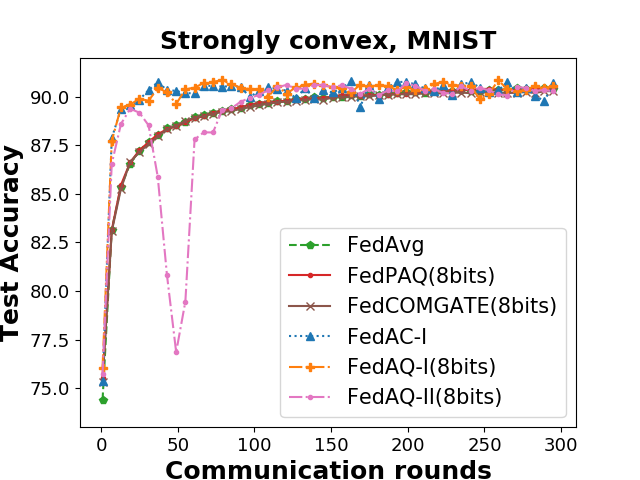
\includegraphics[width=0.31\textwidth]{submissions/YeojoonYoun/figure/accuracy_iid_comm_str_cvx.png}
    %\caption{DCGAN}
    }
    \end{subfigure}
    % Figure 1
    \begin{subfigure}[]{
    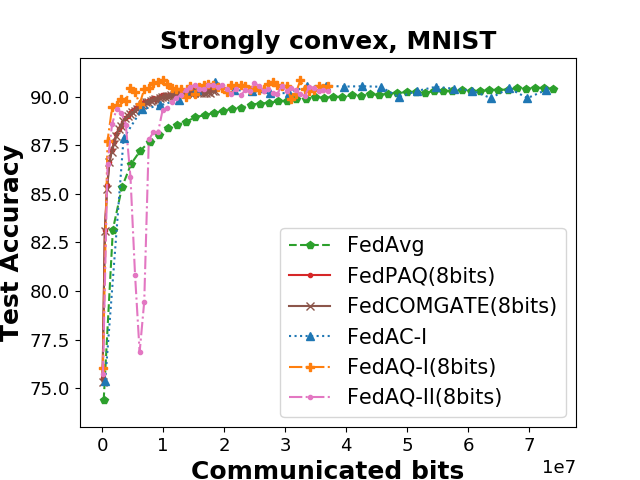
\includegraphics[width=0.31\textwidth]{submissions/YeojoonYoun/figure/accuracy_iid_bits_str_cvx.png}
    %\caption{DCGAN}
    }
    \end{subfigure}
    %\quad
    % Figure 2
    \begin{subfigure}[]{
    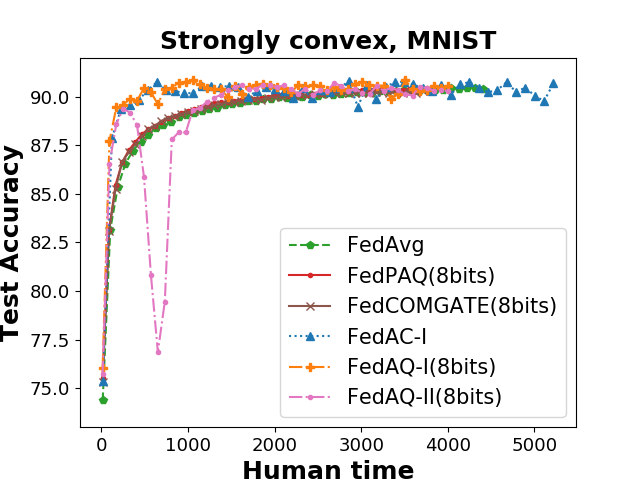
\includegraphics[width=0.31\textwidth]{submissions/YeojoonYoun/figure/accuracy_iid_time_str_cvx.png}
    %\caption{OKGAN}
    }
    \end{subfigure}

    \setcounter{subfigure}{0}
    % Figure 0
    \begin{subfigure}[]{
    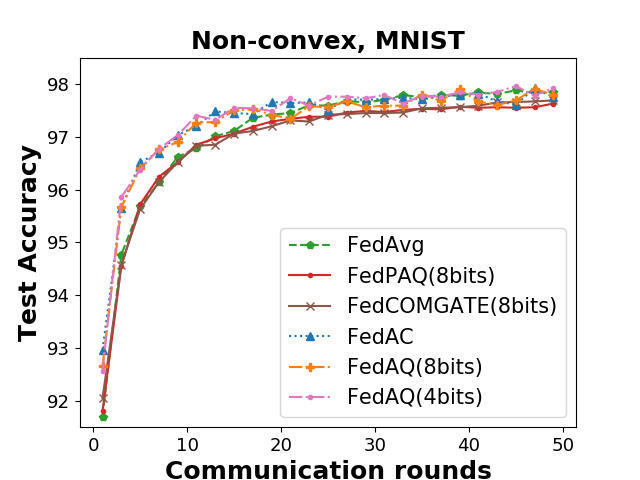
\includegraphics[width=0.31\textwidth]{submissions/YeojoonYoun/figure/accuracy_iid_comm_localstep_100_2.png}
    %\caption{DCGAN}
    }
    \end{subfigure}
    % Figure 1
    \begin{subfigure}[]{
    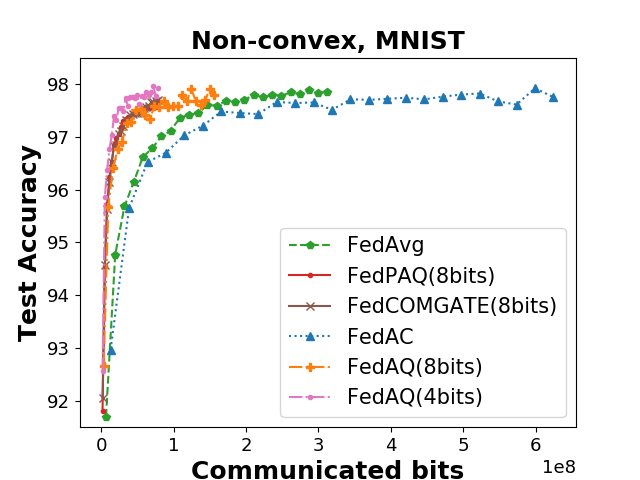
\includegraphics[width=0.31\textwidth]{submissions/YeojoonYoun/figure/accuracy_iid_bits_localstep_100_2.png}
    %\caption{DCGAN}
    }
    \end{subfigure}
    %\quad
    % Figure 2
    \begin{subfigure}[]{
    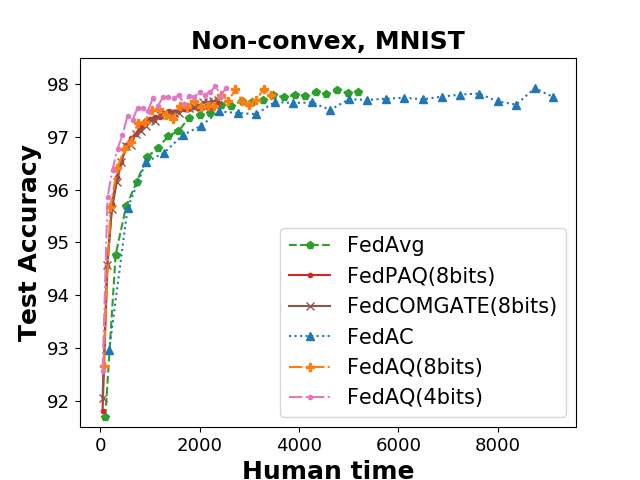
\includegraphics[width=0.31\textwidth]{submissions/YeojoonYoun/figure/accuracy_iid_time_localstep_100_2.png}
    %\caption{OKGAN}
    }
    \end{subfigure}
    \caption{Comparing FedAQ with FedAvg, FedPAQ, FedCOMGATE, and FedAC on MNIST with Strongly Convex Settings (first row) and Non-Convex Settings (second row). We observe how the test accuracy changes across communication rounds (first column), communicated bits (second column), and human time (third column). FedAQ-I outperforms other algorithms in all plots for strongly convex settings. Moreover, FedAQ(4bits) outperforms other algorithms in all plots for non-convex settings.}
    \label{mnist_graph}
\end{figure*}
%\FloatBarrier

\begin{figure*}[hbt!]%[!htbp]
    \centering
    % Figure 0
    \begin{subfigure}[]{
    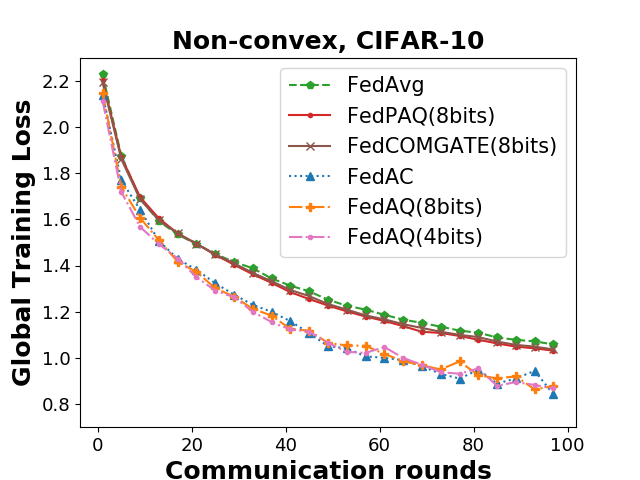
\includegraphics[width=0.31\textwidth]{submissions/YeojoonYoun/figure/loss_iid_comm_cnn_step100.png}
    %\caption{DCGAN}
    }
    \end{subfigure}
    % Figure 1
    \begin{subfigure}[]{
    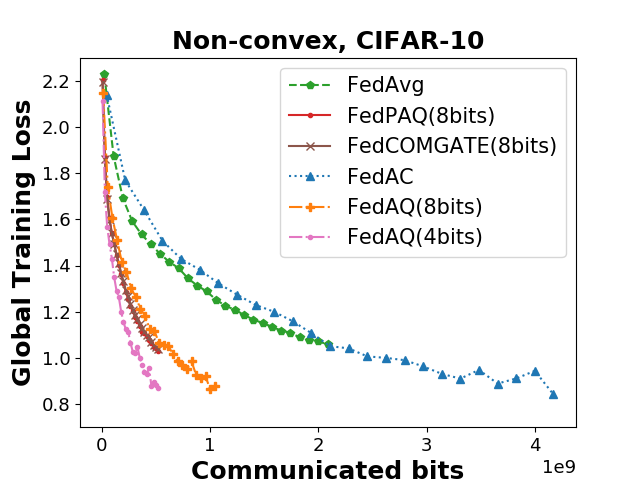
\includegraphics[width=0.31\textwidth]{submissions/YeojoonYoun/figure/loss_iid_bits_cnn_step100.png}
    %\caption{DCGAN}
    }
    \end{subfigure}
    %\quad
    % Figure 2
    \begin{subfigure}[]{
    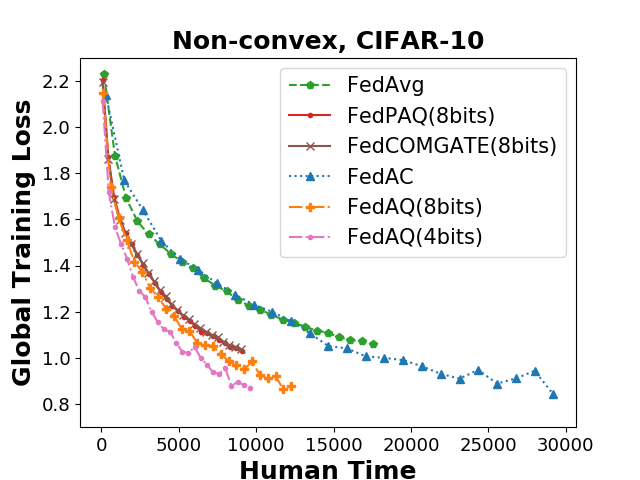
\includegraphics[width=0.31\textwidth]{submissions/YeojoonYoun/figure/loss_iid_time_cnn_step100.png}
    %\caption{OKGAN}
    }
    \end{subfigure}

    \setcounter{subfigure}{0}
    % Figure 0
    \begin{subfigure}[]{
    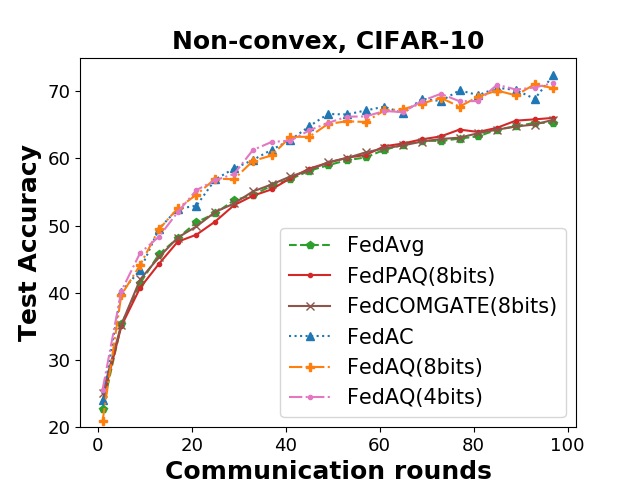
\includegraphics[width=0.31\textwidth]{submissions/YeojoonYoun/figure/accuracy_iid_comm_cnn_step100.png}
    %\caption{DCGAN}
    }
    \end{subfigure}
    % Figure 1
    \begin{subfigure}[]{
    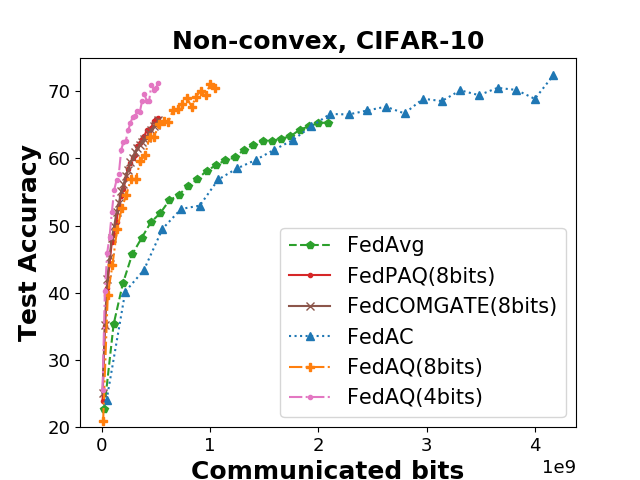
\includegraphics[width=0.31\textwidth]{submissions/YeojoonYoun/figure/accuracy_iid_bits_cnn_step100.png}
    %\caption{DCGAN}
    }
    \end{subfigure}
    %\quad
    % Figure 2
    \begin{subfigure}[]{
    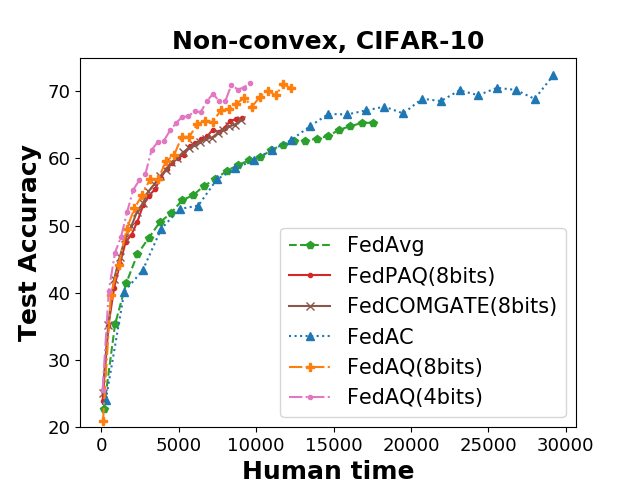
\includegraphics[width=0.31\textwidth]{submissions/YeojoonYoun/figure/accuracy_iid_time_cnn_step100.png}
    %\caption{OKGAN}
    }
    \end{subfigure}
    \caption{Comparing FedAQ with FedAvg, FedPAQ, FedCOMGATE, and FedAC on CIFAR-10. We observe how the global training loss and test accuracy change across communication rounds (first column), communicated bits (second column), and human time (third column). We use a CNN model for CIFAR-10. Similar to the MNIST experiment, FedAQ (4 bits) outperforms all other algorithms in every case.}
    \label{cifar10_graph}
\end{figure*}

